\chapter{Plan of Remaining Work}

\section{Remaining work}

In terms of work remaining, the vast majority of my research and algorithm development has been completed. Only as testing progresses and inevitable changes are be required, will there need to be more research undertaken.

\subsection{Algorithm and Java API Implementation}

The algorithm and mathematical foundation for this project has been established and explained. I've completed a significant amount of the Java API which implements the algorithm and also classes which deal with data persistence, sorting and topic classification. I have yet to test the API rigorously and make alterations to it which may be required for its integration with the demonstration app. 

\subsection{Demonstration Application}

The demonstration application has not yet been implemented. This is the main task of the coming term. I need to finish testing and refining the Java API until it works as expected. A skeleton user interface will be made separately from the API and simultaneously with the API testing. The application will then integrate with the API and I'll first test the algorithm using fake test data. Once this is working I'll use real data sources such as Twitter and Facebook accounts, and  tasks and appointments from the device. 

\section{Planning and Contingency}

After returning from Christmas there will be three weeks of revision and exams, after which 15 weeks remain. I've allocated generous slots for the completion of each of the remaining tasks, and two weeks contingency time before the deadline. 

\subsection{Algorithm and Java API Implementation}

The algorithm and Java API has been largely implemented, but significant amounts still remain. I've allocated a remaining 11 weeks in total for the completion of the API and the demonstration app, to allow for testing and the write up of the final report before the deadline. Over the Christmas break and shortly afterwards, I will be completing the API and validating its results. In terms of contingency planning, should this process overrun significantly, it may be required that a console or desktop demonstration application should be used as opposed to a prototype mobile application. 

\subsection{Demonstration Application}

From early February, the development of the mobile application will begin. This will run alongside the write up of the final report, and continued testing will inform the validation process throughout, such that before the Easter before the deadline, an entire system will have been researched, designed, implemented and tested. This will leave time for a thorough analysis and evaluation of my findings, and for though concerning future work. 


\begin{figure}[p]
    \makebox[\linewidth]{
        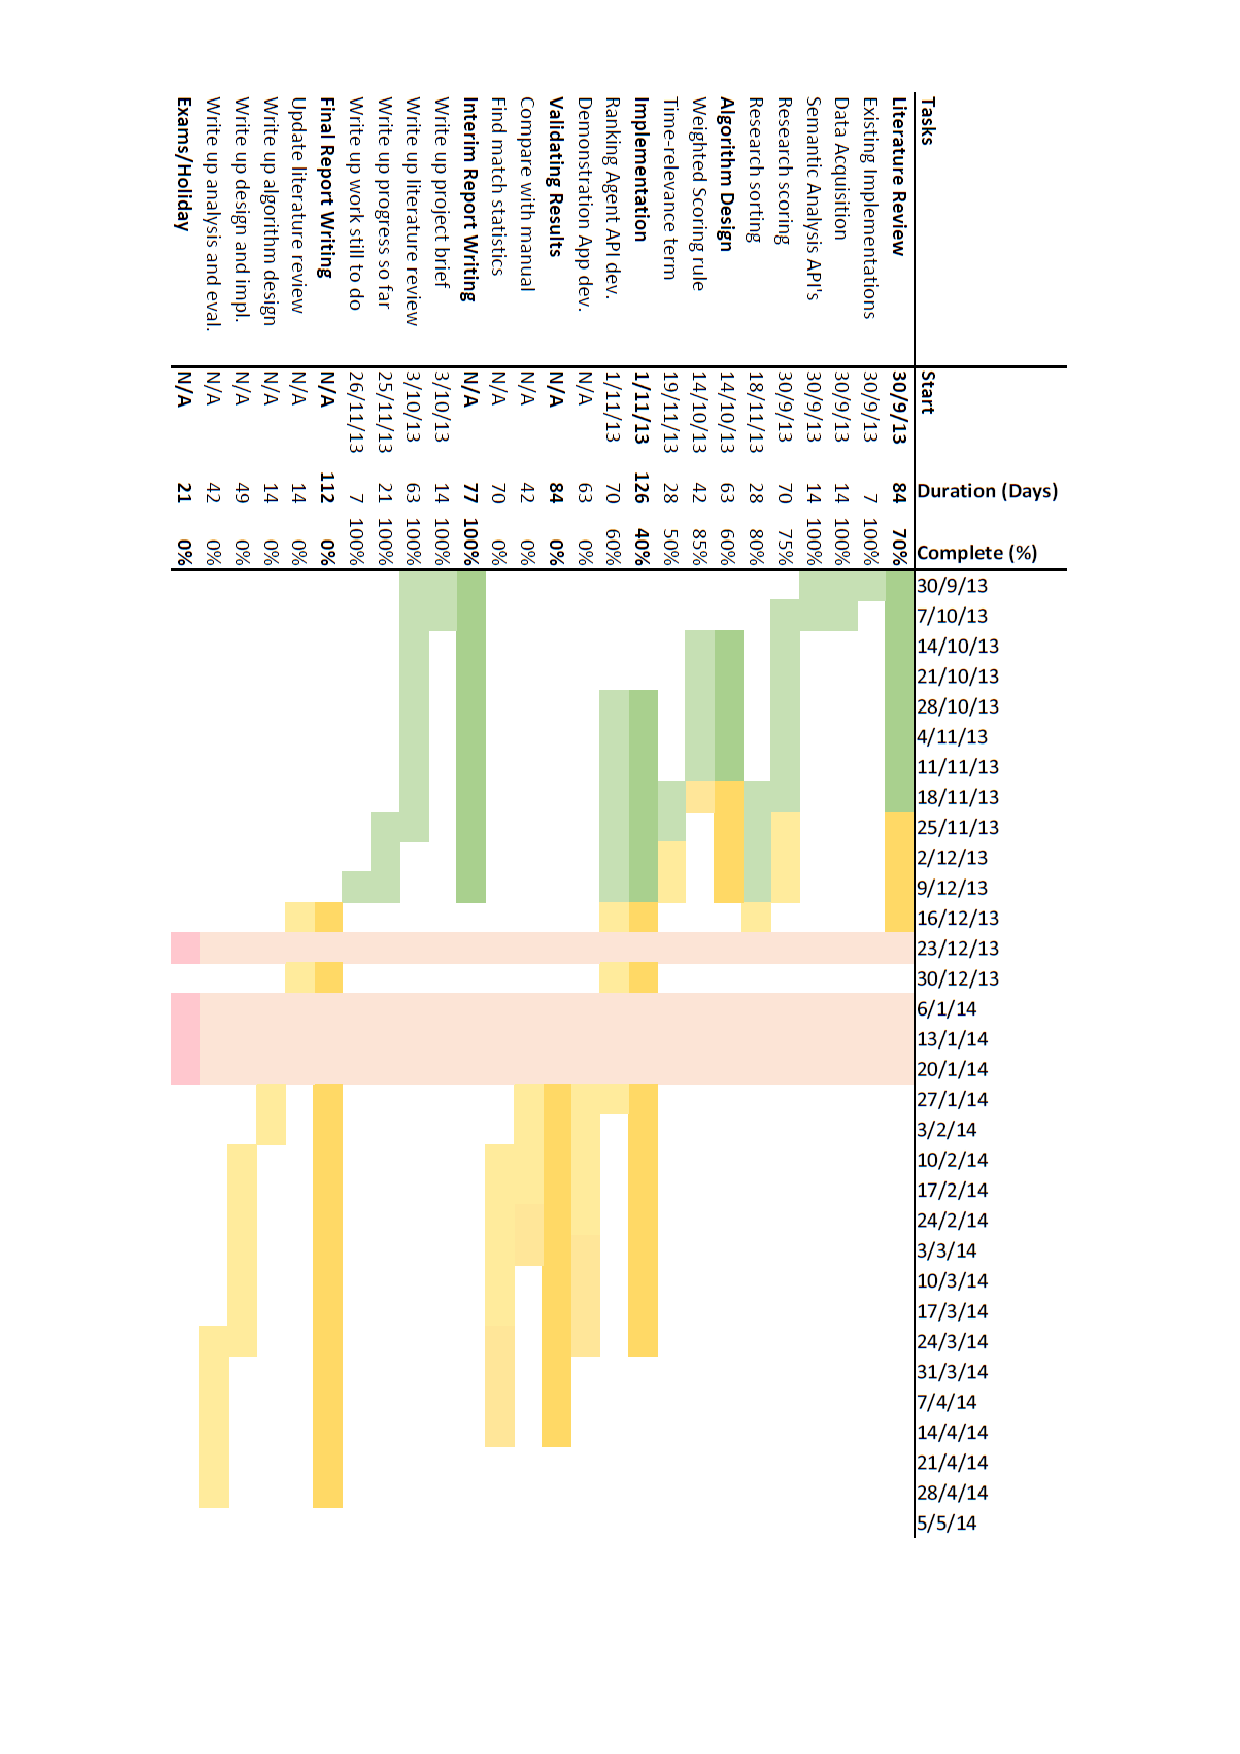
\includegraphics[width=1.3\linewidth]{images/gantt2.pdf}
    }
    \caption{Gantt Chart}
\end{figure}


